\documentclass[professionalfonts]{beamer}

\usepackage{pgfplots}
\usepackage{pgfplotstable}
\pgfplotsset{compat=newest}
\usepgfplotslibrary{ternary}
\usepackage{color, colortbl}

\usepackage{lmodern}
\usepackage{cmbright}
\usepackage{moreverb}
\usepackage[protrusion=true,expansion=true]{microtype}
\usepackage[normalem]{ulem} 
\usepackage{colortbl}
\usepackage{booktabs}
\usepackage{tikz}
\usepackage{amsmath}
\usepackage[scaled]{helvet}

\setbeamertemplate{navigation symbols}{}

\definecolor{STRCOL}{RGB}{251, 128, 114}

\setbeamercolor*{normal text}{fg=black} 
\setbeamercolor*{alerted text}{fg=red} 
\setbeamercolor*{example text}{fg=black} 
\setbeamercolor*{structure}{fg=STRCOL!50!black,bg=white} 
\setbeamercolor*{footline}{fg=black}

\setbeamercolor*{block title}{fg=STRCOL!50!black}
\setbeamercolor*{block body}{fg=black}

\setbeamercolor*{block title example}{fg=green!60!black}
\setbeamercolor*{block body example}{fg=black}
\setbeamerfont{block title}{family=\bfseries}
\setbeamerfont{structure}{family=\bfseries}
\setbeamercolor*{normal text}{fg=black} 

\setbeamertemplate{background canvas}[vertical shading][top=blue!2!white,middle=white,bottom=white]

\newlength\barheight\setlength\barheight{\paperheight}
\divide\barheight by 12
%\setbeamerfont{title}{size=\huge,family=\sffamily}
\setbeamerfont{frametitle}{shape=\bfseries,size=\large}
%\setbeamerfont{subtitle}{size=\Large,shape=\itshape}
%\setbeamerfont{author}{shape=\bfseries,family=\sffamily}
%\setbeamerfont{institute}{size=\small,family=\sffamily}
%\setbeamertemplate{itemize items}[triangle] 
\setbeamertemplate{title page}
{
\vskip 5pt
{\sffamily\tiny\insertdate}
\vskip0pt plus 1filll
\vbox to 2\barheight{%
{\usebeamerfont{title}\usebeamercolor[fg]{title}\inserttitle}}%
\vskip -2em
\ifx\insertsubtitle\@empty\else%
\vskip 1em
{\usebeamerfont{subtitle}\usebeamercolor[fg]{subtitle}\insertsubtitle\par}
\fi
\vskip0pt plus 1filll
{\usebeamerfont{author}\usebeamercolor[fg]{author}\insertauthor}
\vskip4pt
{\usebeamerfont{institute}\usebeamercolor[fg]{institute}\insertinstitute}
\vskip 1em
} 

\setbeamertemplate{frametitle}{%
\begin{flushright}%
\insertframetitle%
\end{flushright}%
\vskip -1em
}

%\insertpagenumber~de~\insertpresentationendpage
%% Color brewer colormaps for pgfplots

\pgfplotsset{
    colormap={spectral}{
		rgb255(0cm)=(158,1,66); 
		rgb255(1cm)=(213,62,79);
		rgb255(2cm)=(244,109,67);
		rgb255(3cm)=(253,174,97);
		rgb255(4cm)=(254,224,139);
		rgb255(5cm)=(255,255,191);
		rgb255(6cm)=(230,245,152);
		rgb255(7cm)=(171,221,164);
		rgb255(8cm)=(102,194,165);
		rgb255(9cm)=(50,136,189);
		rgb255(10cm)=(94,79,162);}
	}

\pgfplotsset{
    colormap={PuBu}{
		rgb255(0cm)=(241,238,246);
		rgb255(1cm)=(4,90,141);}
	}

\pgfplotsset{
    colormap={BuGn}{
		rgb255(0cm)=(237,248,251);
		rgb255(1cm)=(0,109,44);}
	}

\definecolor{RYB1}{RGB}{141, 211, 199}
\definecolor{RYB2}{RGB}{255, 255, 179}
\definecolor{RYB3}{RGB}{190, 186, 218}
\definecolor{RYB4}{RGB}{251, 128, 114}
\definecolor{RYB5}{RGB}{128, 177, 211}
\definecolor{RYB6}{RGB}{253, 180, 98}
\definecolor{RYB7}{RGB}{179, 222, 105}

\pgfplotscreateplotcyclelist{colorbrewer-RYB}{
{RYB1!50!black,fill=RYB1},
{RYB2!50!black,fill=RYB2},
{RYB3!50!black,fill=RYB3},
{RYB4!50!black,fill=RYB4},
{RYB5!50!black,fill=RYB5},
{RYB6!50!black,fill=RYB6},
{RYB7!50!black,fill=RYB7},
}

\definecolor{grey}{rgb}{0.6,0.6,0.6}
\definecolor{orange}{RGB}{255,140,0}

\title{Food web motifs and the functioning of complex ecosystems}
\author{Timoth\'ee Poisot}
\institute{Theoretical Ecosystem Ecology, UQAR}
\date{\today}

\begin{document}

\frame[plain]{\titlepage}

\begin{frame}{Biodiversity and ecosystem functioning}
	\begin{center}
	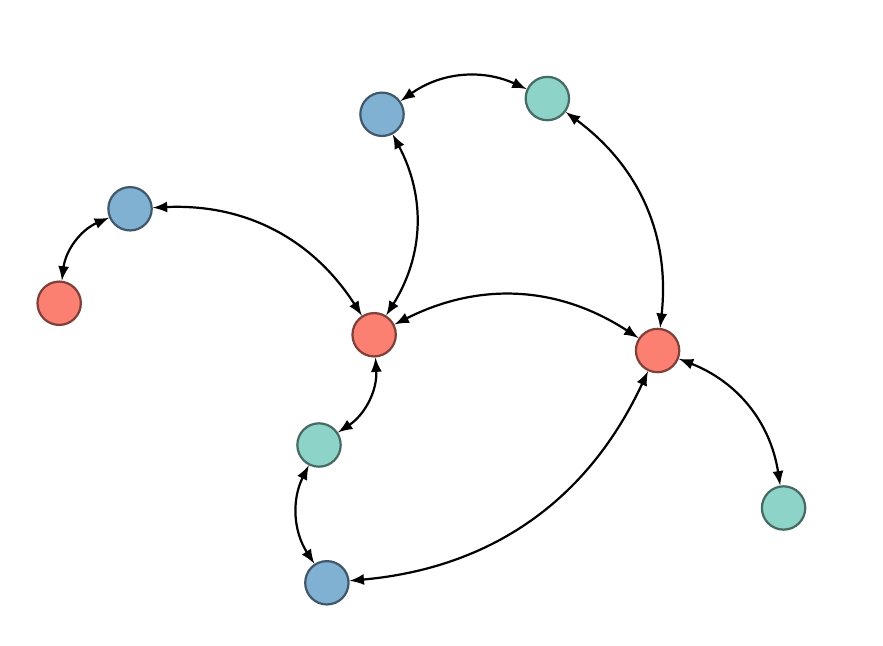
\begin{tikzpicture}[>=latex,text height=1.5ex,text depth=0.25ex]
		%\draw[help lines, draw=none] (0,0) grid (10.5,7.5);
		\path[use as bounding box] (0,0) rectangle(10.5,7.5);
		\tikzstyle{every node}=[draw,minimum size = .4cm,circle,draw=RYB1!50!black,fill=RYB1]	
		\tikzstyle{every path}=[solid,thick]
		%% First species
		\draw (3.7,2.2) node (a) {};
		\draw (9.6,1.4) node (b) {};
		\draw (6.6,6.6) node (c) {};
		%% Second species
		\draw <2-> (0.4,4.0) node [draw=RYB4!50!black,fill=RYB4] (d) {};
		\draw <2-> (4.4,3.6) node [draw=RYB4!50!black,fill=RYB4] (e) {};
		\draw <2-> (8.0,3.4) node [draw=RYB4!50!black,fill=RYB4] (f) {};
		%% Third species
		\draw <3-> (1.3,5.2) node [draw=RYB5!50!black,fill=RYB5] (g) {};
		\draw <3-> (4.5,6.4) node [draw=RYB5!50!black,fill=RYB5] (h) {};
		\draw <3-> (3.8,0.45) node [draw=RYB5!50!black,fill=RYB5] (i) {};
		%% Arrows
		\path <4> [<->] (g) edge [bend right] (d);
		\path <4> [<->] (g) edge [bend left] (e);
		\path <4> [<->] (h) edge [bend left] (c);
		\path <4> [<->] (e) edge [bend left] (a);
		\path <4> [<->] (i) edge [bend left] (a);
		\path <4> [<->] (i) edge [bend right] (f);
		\path <4> [<->] (b) edge [bend right] (f);
		\path <4> [<->] (e) edge [bend left] (f);
		\path <4> [<->] (e) edge [bend right] (h);
		\path <4> [<->] (f) edge [bend right] (c);
	\end{tikzpicture}
	\end{center}
\end{frame}


\begin{frame}{Three-species motifs: capturing complexity}
	\begin{center}
		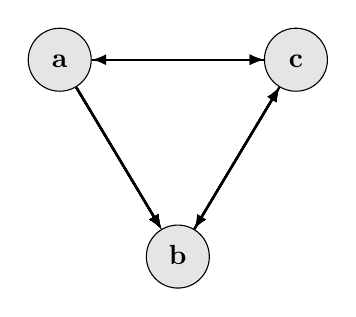
\begin{tikzpicture}[>=latex,text height=1.5ex,text depth=0.25ex]
			%% \draw[help lines] (0,0) grid (4,3);
			\tikzstyle{every node}=[draw,minimum size = .8cm,circle,draw=black,fill=black!10]	
			%% Web
			\draw (0,3) node (a) {\textbf{a}};
			\draw (1.5,0.5) node (b) {\textbf{b}};
			\draw (3,3) node (c) {\textbf{c}};
			%% Motif S1
			\draw <1> [solid,thick,->] (a) -- (b);
			\draw <1> [solid,thick,->] (b) -- (c);
			%% Motif S2
			\draw <2> [solid,thick,->] (a) -- (b);
			\draw <2> [solid,thick,->] (b) -- (c);
			\draw <2> [solid,thick,->] (a) -- (c);
			%% Motif S3
			\draw <3> [solid,thick,->] (a) -- (b);
			\draw <3> [solid,thick,->] (b) -- (c);
			\draw <3> [solid,thick,->] (c) -- (a);
			%% Motif S4
			\draw <4> [solid,thick,->] (a) -- (b);
			\draw <4> [solid,thick,->] (c) -- (b);
			%% Motif S5
			\draw <5> [solid,thick,->] (a) -- (b);
			\draw <5> [solid,thick,->] (a) -- (c);
		\end{tikzpicture}
	\end{center}
\end{frame}

\begin{frame}{Three-species motifs: capturing complexity}
	\begin{center}
		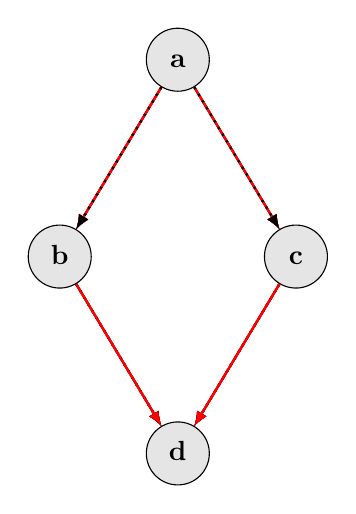
\begin{tikzpicture}[>=latex,text height=1.5ex,text depth=0.25ex]
			%% \draw[help lines] (0,0) grid (3,6);
			\tikzstyle{every node}=[draw,minimum size = .8cm,circle,draw=black,fill=black!10]
			\draw (0,3) node (b) {\textbf{b}};
			\draw (1.5,5.5) node (a) {\textbf{a}};
			\draw (3,3) node (c) {\textbf{c}};
			\draw (1.5,0.5) node (d) {\textbf{d}};
			%% Arrows on slide 1
			\draw <1> [solid,thick,->] (a) -- (b);
			\draw <1> [solid,thick,->] (b) -- (d);
			\draw <1> [solid,thick,->] (a) -- (c);
			\draw <1> [solid,thick,->] (c) -- (d);
			%% LFC 1
			\draw <2> [solid,thick,->,red] (a) -- (b);
			\draw <2> [solid,thick,->,red] (b) -- (d);
			\draw <2> [dotted,thick,->] (a) -- (c);
			\draw <2> [dotted,thick,->] (c) -- (d);
			%% LFC 2
			\draw <3> [dotted,thick,->] (a) -- (b);
			\draw <3> [dotted,thick,->] (b) -- (d);
			\draw <3> [solid,thick,->,red] (a) -- (c);
			\draw <3> [solid,thick,->,red] (c) -- (d);
			%% Apparent competition
			\draw <4> [solid,thick,->,red] (a) -- (b);
			\draw <4> [solid,thick,->,red] (a) -- (c);
			\draw <4> [dotted,thick,->] (b) -- (d);
			\draw <4> [dotted,thick,->] (c) -- (d);
			%% Exploitative competition
			\draw <5> [dotted,thick,->] (a) -- (b);
			\draw <5> [dotted,thick,->] (a) -- (c);
			\draw <5> [solid,thick,->,red] (b) -- (d);
			\draw <5> [solid,thick,->,red] (c) -- (d);
		\end{tikzpicture}
	\end{center}
\end{frame}

\begin{frame}{Dynamical meaning of first-order motifs}
	\begin{center}
	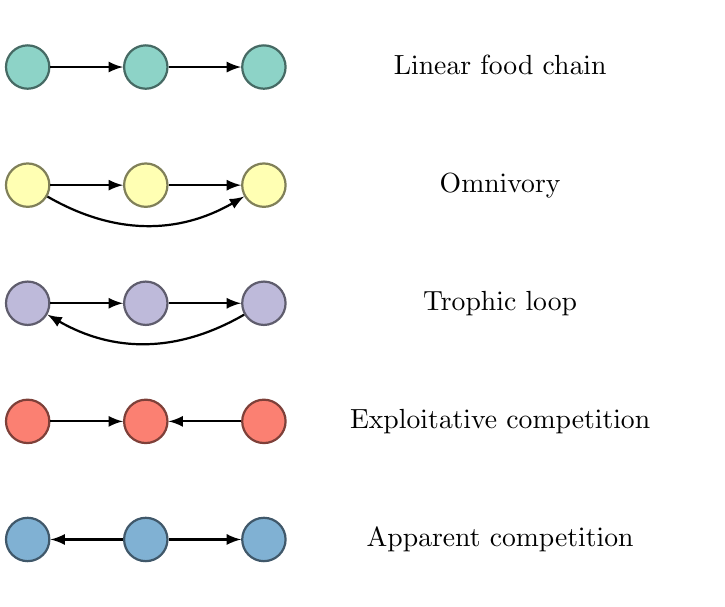
\begin{tikzpicture}[>=latex,text height=1.5ex,text depth=0.25ex]
		% \draw[help lines] (0,0) grid (8.5,7);
		\path[use as bounding box] (0,0) rectangle(8.5,7);
		\tikzstyle{every node}=[draw,minimum size = .3cm,circle,draw=none,fill=black!10]
		\tikzstyle{every path}=[solid,thick]
		
		%% Motif one
		\draw (0,6.5) node [draw=RYB1!50!black,fill=RYB1] (m11) {};
		\draw (1.5,6.5) node [draw=RYB1!50!black,fill=RYB1] (m12) {};
		\draw (3,6.5) node [draw=RYB1!50!black,fill=RYB1] (m13) {};
		\path [->] (m11) edge (m12);
		\path [->] (m12) edge (m13);
		\draw (6,6.5) node [draw = none, fill=none] (lfc) {Linear food chain};
		
		%% Motif two
		\draw <2-> (0,5) node [draw=RYB2!50!black,fill=RYB2] (m21) {};
		\draw <2-> (1.5,5) node [draw=RYB2!50!black,fill=RYB2] (m22) {};
		\draw <2-> (3,5) node [draw=RYB2!50!black,fill=RYB2] (m23) {};
		\path <2-> [->] (m21) edge (m22);
		\path <2-> [->] (m22) edge (m23);
		\path <2-> [->] (m21) edge [bend right] (m23);
		\draw <2-> (6,5) node [draw = none, fill=none] (omn) {Omnivory};
		
		%% Motif three
		\draw <3-> (0,3.5) node [draw=RYB3!50!black,fill=RYB3] (m31) {};
		\draw <3-> (1.5,3.5) node [draw=RYB3!50!black,fill=RYB3] (m32) {};
		\draw <3-> (3,3.5) node [draw=RYB3!50!black,fill=RYB3] (m33) {};
		\path <3-> [->] (m31) edge (m32);
		\path <3-> [->] (m32) edge (m33);
		\path <3-> [->] (m33) edge [bend left] (m31);
		\draw <3-> (6,3.5) node [draw = none, fill=none] (tl) {Trophic loop};
		
		%% Motif four
		\draw <4-> (0,2) node [draw=RYB4!50!black,fill=RYB4] (m41) {};
		\draw <4-> (1.5,2) node [draw=RYB4!50!black,fill=RYB4] (m42) {};
		\draw <4-> (3,2) node [draw=RYB4!50!black,fill=RYB4] (m43) {};
		\path <4-> [->] (m41) edge (m42);
		\path <4-> [->] (m43) edge (m42);
		\draw <4-> (6,2) node [draw = none, fill=none] (exc) {Exploitative competition};
		
		%% Motif five
		\draw <5-> (0,0.5) node [draw=RYB5!50!black,fill=RYB5] (m51) {};
		\draw <5-> (1.5,0.5) node [draw=RYB5!50!black,fill=RYB5] (m52) {};
		\draw <5-> (3,0.5) node [draw=RYB5!50!black,fill=RYB5] (m53) {};
		\path <5-> [->] (m52) edge (m51);
		\path <5-> [->] (m52) edge (m53);
		\draw <5-> (6,0.5) node [draw = none, fill=none] (pac) {Apparent competition};
		
	\end{tikzpicture}
	\end{center}
\end{frame}

\begin{frame}{Variation in motif composition}
	\begin{center}
		\begin{tikzpicture}
			\begin{axis}[height=7cm, width=8.5cm,
				stack plots=y, enlargelimits=false,
				const plot, area style,
				ymin=0, ymax=1,
				xlabel = Network number, ylabel = Motif frequency,
				cycle list name=colorbrewer-RYB,
				legend style={
					area legend,
					at={(1.05,0.5)},
					anchor=west,
					legend columns=1}
			]
			\addplot table [x=prank, y=S1] {../cleaned.dat} \closedcycle;
			\addplot table [x=prank, y=S2] {../cleaned.dat} \closedcycle;
			\addplot table [x=prank, y=S3] {../cleaned.dat} \closedcycle;
			\addplot table [x=prank, y=S4] {../cleaned.dat} \closedcycle;
			\addplot table [x=prank, y=S5] {../cleaned.dat} \closedcycle;
			\legend{S1,S2,S3,S4,S5};
			
			\end{axis}
		\end{tikzpicture}
	\end{center}
\end{frame}

\begin{frame}{The question}
	\begin{center}
		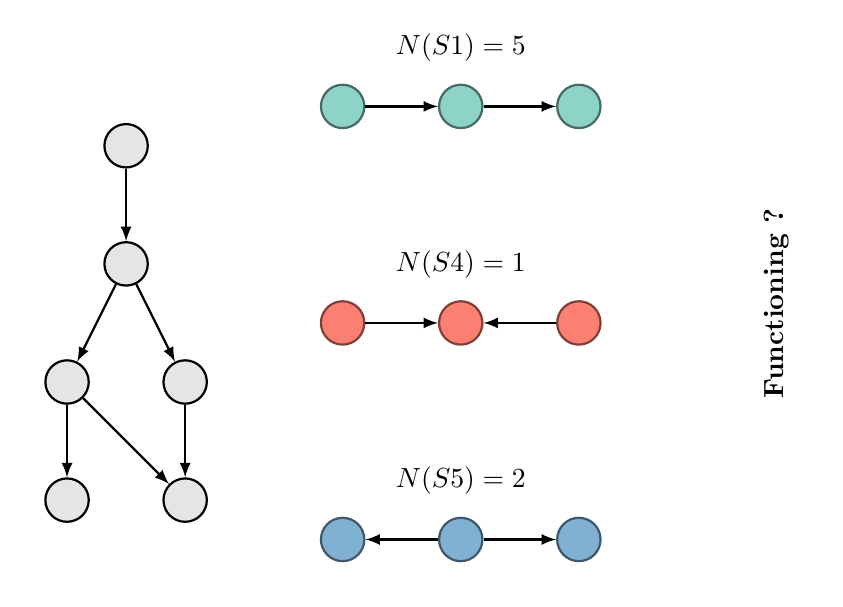
\begin{tikzpicture}[>=latex,text height=1.5ex,text depth=0.25ex]
				%\draw[help lines] (0,0) grid (10,7);
				\tikzstyle{every node}=[draw,minimum size = .15cm,circle,draw=black,fill=black!10]
				\tikzstyle{every path}=[solid,thick]
				\path[use as bounding box] (0,0) rectangle(10,7);
				%% Full food web
				\draw (0.5,1) node (a) {\textbf{}};
				\draw (2,1) node (b) {\textbf{}};
				\draw (0.5,2.5) node (c) {\textbf{}};
				\draw (2,2.5) node (d) {\textbf{}};
				\draw (1.25,4) node (e) {\textbf{}};
				\draw (1.25,5.5) node (f) {\textbf{}};
				\path [->] (f) edge (e);
				\path [->] (e) edge (c);
				\path [->] (e) edge (d);
				\path [->] (c) edge (a);
				\path [->] (c) edge (b);
				\path [->] (d) edge (b);
				
				%% Motifs 1
				\draw <2-> (4, 6) node [draw=RYB1!50!black,fill=RYB1] (m11) {};
				\draw <2-> (5.5, 6) node [draw=RYB1!50!black,fill=RYB1] (m12) {};
				\draw <2-> (7, 6) node [draw=RYB1!50!black,fill=RYB1] (m13) {};
				\path <2-> [->] (m11) edge (m12);
				\path <2-> [->] (m12) edge (m13);
				\draw <2-> (5.5, 6.75) node [draw=none, fill=none] (tm1) {$N(S1) = 5$};
				
				%% Motifs 2
				\draw <3-> (4, 3.25) node [draw=RYB4!50!black,fill=RYB4] (m21) {};
				\draw <3-> (5.5, 3.25) node [draw=RYB4!50!black,fill=RYB4] (m22) {};
				\draw <3-> (7, 3.25) node [draw=RYB4!50!black,fill=RYB4] (m23) {};
				\path <3-> [->] (m21) edge (m22);
				\path <3-> [->] (m23) edge (m22);
				\draw <3-> (5.5, 4) node [draw=none, fill=none] (tm2) {$N(S4) = 1$};
				
				%% Motifs 3
				\draw <4-> (4, 0.5) node [draw=RYB5!50!black,fill=RYB5] (m31) {};
				\draw <4-> (5.5, 0.5) node [draw=RYB5!50!black,fill=RYB5] (m32) {};
				\draw <4-> (7, 0.5) node [draw=RYB5!50!black,fill=RYB5] (m33) {};
				\path <4-> [->] (m32) edge (m31);
				\path <4-> [->] (m32) edge (m33);
				\draw <4-> (5.5, 1.25) node [draw=none, fill=none] (tm3) {$N(S5) = 2$};
				
				%% Functioning ?
				\draw <5-> (9.5, 3.5) node [rotate = 90, draw=none, fill=none] (FUNC) {\bfseries Functioning ?};
				
			\end{tikzpicture}
		\end{center}
\end{frame}


\begin{frame}{The model}
	\begin{align}
		\frac{dN_{i}}{dt} &= N_{i}\left[r\left(1-\frac{N_{i}}{K}\right) - \sum_{j \in pred} \alpha N_{j}\right] \\
		\frac{dN_{i}}{dt} &= N_{i}\left[\sum_{j \in prey} \beta N_{j} - \sum_{j \in pred} \alpha N_{j} - \delta\right]
	\end{align}
\end{frame}

\begin{frame}{The model}
	\begin{center}
		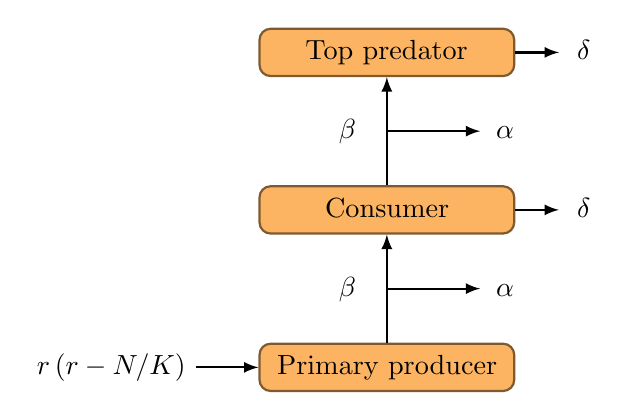
\begin{tikzpicture}[>=latex,text height=1.5ex,text depth=0.25ex]
			%\draw[help lines] (0,0) grid (8,5);
			\tikzstyle{every node}=[draw,minimum size=.6cm,rectangle,fill=RYB6,draw=RYB6!50!black]	
			\tikzstyle{every path}=[solid,thick]
			
			%% Species
			\draw (4.5,0.5) node [text width = 3cm, text centered, rounded corners] (pp) {Primary producer};
			\draw (4.5,2.5) node [text width = 3cm, text centered, rounded corners] (co) {Consumer};
			\draw (4.5,4.5) node [text width = 3cm, text centered, rounded corners] (tp) {Top predator};
			
			%% Interactions
			\path [->] (pp) edge (co);
			\path [->] (co) edge (tp);
			
			%% Biomass gain and loss			
			\draw (1,0.5) node [draw=none,fill=none] (ipp) {$r\left(r-N/K\right)$};
			\path [->] (ipp) edge (pp);
			
			\draw (7,2.5) node [draw=none,fill=none] (dco) {$\delta$};
			\path [->] (co) edge (dco);
			
			\draw (6,1.5) node [draw=none,fill=none] (aco) {$\alpha$};
			\path [->] (4.5,1.5) edge (aco);
			
			\draw (7,4.5) node [draw=none,fill=none] (dtp) {$\delta$};
			\path [->] (tp) edge (dtp);
			
			\draw (6,3.5) node [draw=none,fill=none] (atp) {$\alpha$};
			\path [->] (4.5,3.5) edge (atp);
			
			\draw (4,1.5) node [draw=none,fill=none] (bco) {$\beta$};
			\draw (4,3.5) node [draw=none,fill=none] (btp) {$\beta$};
			
		\end{tikzpicture}
	\end{center}
\end{frame}

\begin{frame}{Simulations}
	\begin{itemize}
		\item Each species starts with $N_{i} \in [0,1]$, at random
		\item We run the system well over equilibrium ($10^{4}$ time steps)
		\item We record the total biomass of the system
		\item Repeat 10 times for each of the 180 webs
		\item Average over the 10 replicates presented in the figures
	\end{itemize}
\end{frame}

\begin{frame}{Exploitative competition}
	\begin{center}
		\begin{tikzpicture}
		\begin{axis}[height=7cm, width=8.5cm,
			xmin = 0, xmax = 0.8, xlabel=Frequency of motif S4,
			ymin = 0, ymax = 1.5, ylabel=Mean biomass,
			grid=major]
			\addplot[only marks, mark=*] table [x=S4,y=bmm] {../cleaned.dat};
%			\addplot[mark=none, thick] table [x =S4, y={create col/linear regression={y=bmm}}] {../cleaned.dat};
			%% MOTIF S4
			\draw (axis cs:0.65,1.35) node [draw=RYB4!50!black,fill=RYB4, circle] (S1) {};
			\draw (axis cs:0.75,1.35) node [draw=RYB4!50!black,fill=RYB4, circle] (S2) {};
			\draw (axis cs:0.7,1.15) node [draw=RYB4!50!black,fill=RYB4, circle] (S3) {};
			\path [->] (S1) edge (S3);
			\path [->] (S2) edge (S3);
		\end{axis}
		\end{tikzpicture}
	\end{center}
\end{frame}

\begin{frame}{Apparent competition}
	\begin{center}
		\begin{tikzpicture}
		\begin{axis}[height=7cm, width=8.5cm,
			xmin = 0, xmax = 0.8, xlabel=Frequency of motif S5,
			ymin = 0, ymax = 1.5, ylabel=Mean biomass,
			grid=major]
			\addplot[only marks, mark=*] table [x=S5,y=bmm] {../cleaned.dat};
%			\addplot[mark=none, thick] table [x=S5, y={create col/linear regression={y=bmm}}] {../cleaned.dat};
			%% MOTIF S4
			\draw (axis cs:0.05,1.15) node [draw=RYB5!50!black,fill=RYB5, circle] (S1) {};
			\draw (axis cs:0.15,1.15) node [draw=RYB5!50!black,fill=RYB5, circle] (S2) {};
			\draw (axis cs:0.1,1.35) node [draw=RYB5!50!black,fill=RYB5, circle] (S3) {};
			\path [->] (S3) edge (S1);
			\path [->] (S3) edge (S2);
		\end{axis}
		\end{tikzpicture}
	\end{center}
\end{frame}

\begin{frame}{Types of competition}
	\begin{center}
		\begin{tikzpicture}
			\begin{axis}[height=7cm, width=8.5cm,
				view={0}{90},
				grid = major, colormap name=BuGn,
				colorbar,
				xmin = 0, xmax = 0.8,
				ymin = 0, ymax = 0.8,
				zmin = 0, zmax = 2,
				xlabel = Exploitative competition,
				ylabel = Apparent competition,
				label = Mean biomass]
				\addplot3+ [only marks, mark=*, scatter] table [x=S4,y=S5, z=bmm] {../cleaned.dat};
	%			\addplot3+ [mark=none, thick, color=black] table [x =S4, y={create col/linear regression={y=S5}}] {../cleaned.dat};
			\end{axis}
		\end{tikzpicture}
	\end{center}
\end{frame}

\begin{frame}{Competition type ratio}
	\begin{center}
		\begin{tikzpicture}
		\begin{semilogxaxis}[height=7cm, width=8.5cm,
			xmin = 0.1, xmax = 10, xlabel= log$_{10}$(S4/S5),
			ymin = 0, ymax = 1.5, ylabel=Mean biomass,
			grid=major]
			\addplot[only marks, mark=*] table [x=compratio,y=bmm] {../cleaned.dat};
%			\addplot[mark=none, thick] table [x=S5, y={create col/linear regression={y=bmm}}] {../cleaned.dat};
		\end{semilogxaxis}
		\end{tikzpicture}
	\end{center}
\end{frame}

\begin{frame}{Omnivory decreases biomass production}
	\begin{center}
		\begin{tikzpicture}
		\begin{axis}[height=7cm, width=8.5cm,
			xmin = 0, xmax = 0.2, xlabel=Frequency of motif S2,
			ymin = 0, ymax = 1.5, ylabel=Mean biomass,
			grid=major, xtick = {0,0.1,0.2}]
			\addplot[only marks, mark=*] table [x=S2,y=bmm] {../cleaned.dat};
			%% MOTIF S2
			\draw (axis cs:0.165,1.35) node [draw=RYB2!50!black,fill=RYB2, circle] (S1) {};
			\draw (axis cs:0.165,1.15) node [draw=RYB2!50!black,fill=RYB2, circle] (S2) {};
			\draw (axis cs:0.185,1.25) node [draw=RYB2!50!black,fill=RYB2, circle] (S3) {};
			\path [->] (S1) edge (S2);
			\path [->] (S1) edge (S3);
			\path [->] (S3) edge (S2);
		\end{axis}
		\end{tikzpicture}
	\end{center}
\end{frame}

\begin{frame}{Synthesis of the results -- biomass production}
	\begin{center}
		\begin{tabular}{lrrr}
		  \hline
		 Motif & Df & F value & Pr($>$F) \\ 
		  \hline
			\rowcolor{RYB4} Expl. comp. (S4) & 1 & 1287.82 & *** \\ 
			\rowcolor{RYB2} Omnivory (S2) & 1 & 112.18 & *** \\ 
			\rowcolor{RYB1} Lin. chain (S1) & 1 & 91.22 & *** \\ 
			\rowcolor{RYB3} Loop (S3) & 1 & 26.41 & *** \\ 
			\rowcolor{RYB5} App. comp. (S5) & 1 & 11.69 & *** \\ 
			\hline
			Residuals & 1774 &  &  $R^{2} = 0.46$\\ 
		   \hline
		\end{tabular}
	\end{center}
\end{frame}


\begin{frame}{Synthesis of the results -- productivity}
	\begin{center}
		\begin{tabular}{lrrr}
			\hline
			Motif & Df & F value & Pr($>$F) \\ 
			\hline
			\rowcolor{RYB4} Expl. comp. (S4) & 1 & 1013.00 & *** \\ 
			\rowcolor{RYB1} Lin. chain (S1) & 1 & 258.20 & *** \\ 
			\rowcolor{RYB2} Omnivory (S2) & 1 & 42.69 & *** \\ 
			\rowcolor{RYB5} App. comp. (S5) & 1 & 2.28 & 0.13 \\ 
			\rowcolor{RYB3} Loop (S3) & 1 & 0.53 & 0.46 \\ 
			\hline
			Residuals & 1103 &  &  $R^{2} = 0.54$  \\ 
			\hline
		\end{tabular}
	\end{center}
\end{frame}

\begin{frame}{Biomass production and productivity}
	\begin{center}
		\begin{tikzpicture}
		\begin{axis}[height=7cm, width=8.5cm,
			xlabel=Network,
			ymin = 0, ymax = 1.5, ylabel={ },
			grid=major,
			legend style={
				at={(0.5,0.97)},
         		anchor=north,legend columns=-1
			}]
			\addplot [mark=none, color=RYB4, very thick] table [x=prank,y=bmm] {../cleaned.dat};
			\addlegendentry{Biomass}
			\addplot [mark=none, color=RYB5, very thick] table [x=prank,y=prome] {../cleaned.dat};
			\addlegendentry{Productivity}
		\end{axis}
		\end{tikzpicture}
	\end{center}
\end{frame}

\end{document}
